\documentclass[10pt]{report}            % Report class in 11 points
\parindent0pt  \parskip10pt             % make block paragraphs
\raggedright                            % do not right-justify
\usepackage{amsmath, amssymb, amsthm,graphicx, enumitem, hyperref,gensymb, float} %, threeparttable}
\usepackage[table]{xcolor}
\newcommand{\ro}{\mathcal{R}_0}
\makeatletter
\newcommand*{\centerfloat}{%
  \parindent \z@
  \leftskip \z@ \@plus 1fil \@minus \textwidth
  \rightskip\leftskip
  \parfillskip \z@skip}
\makeatother
%*******************************************************************%
\title{\bf Mayo Pharmacy Optimization Case Study\\
\large Using Discrete Event Simulation}  % Supply information
\author{Justin Hood\\
MSCS 791}              %   for the title page.
\date{\today}                           %   Use current date.
\begin{document}                        % End of preamble, start of text.
\maketitle                              % Print title page.
\pagenumbering{roman}                   % roman page number for toc
\setcounter{page}{2}                    % make it start with "ii"
%\tableofcontents                        % Print table of contents
\newpage
\section*{Abstract}
\addcontentsline{toc}{section}{Abstract}
\section*{Introduction}                % Print a "chapter" heading\
\addcontentsline{toc}{section}{Introduction}
\pagenumbering{arabic}                  % Start text with arabic 1
The use of prescription medication is becoming increasingly commonplace in the United States. In 2013, the average number of prescriptions taken per person was $12.2$, up from $9$ in 1998, a $136\%$ increase over 15 years \cite{georgetown}\cite{statistica}. With this trend in prescription usage continuing to rise, pharmacies are becoming an ever greater presence in the lives of most Americans. As such, pharmacies need to adapt to deal with increasing numbers of orders, as well as increasing the speed and accuracy at which they fill orders in order to remain competitive in an increasingly saturated landscape of pharmacies.  Consequently, pharmacies must adapt their methodologies and staffing requirements in order to optimize efficiency and cost. Obviously, testing different optimization schemas is both expensive and time consuming, so pharmacies have begun to consider computer simulation approaches to optimization as a more cost effective solution.\\\hfill\\
In this case study, we are tasked with both modeling and optimizing the workflow for a prototype pharmacy based on samples of data regarding task duration and incoming order frequency. In addition to the sample data for the pharmacy, we are also given a brief overview of the basic order fulfillment process. Using this information, we shall construct a discrete event simulation model to analyze our so called ``control" case, i.e. the pharmacy described by the basic information. Once this simulation is running and tested, we shall attempt to improve the efficiency over the base case. In order to achieve this goal, we shall attack the optimization on two fronts.
\begin{enumerate}
\item Optimizing task priority within the workflow (picking the best task to pull from)
\item Optimizing staff breakdown (profit optimizing number of pharmacists vs. technicians to employ)
\end{enumerate}
With these optimizations, we hope to develop a sense of what changes could increase the efficiency of the pharmacy, as well as an idea of what variables could be manipulated to further increase the accuracy of our simulation, and improve the pharmacy's function.
\section*{Background}
\addcontentsline{toc}{section}{Background}
In our prototypical example, there are two types of prescription orders that the pharmacy receives, oral and IV, which are handled by two different classes of employee, pharmacists and technicians, who are constrained as to which task they may perform due to legal regulations. In our prototype pharmacy, the proposed process is as follows: As the pharmacy receives orders, they are entered into the system by a technician. Once the order is in the system, it is verified by a pharmacist, and passed to the appropriate area to be prepared by technicians. Upon being filled, the order is again verified by a pharmacist, and then dispensed to the consumer by a technician. As such, we see that there are six basic tasks in the workflow tied to the two different types of orders: order entry, entry verification, oral or IV preparation, prepared order verification, and distribution through the window. As noted before, regulations exist to limit what tasks non-pharmacist level employees may perform. These regulations dictate that of the tasks, the verification tasks may only be performed by the pharmacists, while the remaining tasks can be performed by both pharmacists and technicians. A breakdown of this hierarchy follows in Table \ref{table:tasks}, with pharmacist specific tasks highlighted in red. It should also be noted that in our control case, there exists an additional sub-type of technician, whose sole purpose is to prepare IV orders in an isolated room. This will be explored in greater detail below.
\begin{table}[H]
\centering
\begin{tabular}{|c||c|c|}
\hline
Pharmacist & Technician & IV Technician\\\hline\hline
Order Entry & Order Entry &\\\hline
\cellcolor{red!25}Entry Verification && \\\hline
Oral Drug Preparation & Oral Drug Preparation & \cellcolor{blue!25}IV Drug Preparation\\\hline
\cellcolor{red!25}Preparation Verification &&\\\hline
Distribution & Distribution&\\\hline
\end{tabular}
\caption{Pharmacist vs Technician tasks.}
\label{table:tasks}
\end{table}
With this task breakdown in hand, we consider a graphical representation of the path an order takes within the pharmacy, specifically linked to the tasks described above. Looking at Figure \ref{fig:flowchart}, we see that the process of filling an order is fairly linear, with the only fork in the workflow occurring after the entry verification step. This fork is due to the necessity of establishing an order's type (Oral vs. IV) so it may be put in the appropriate filling queue. In our control pharmacy, all IV orders are filled in an isolated room by an ``IV Technician" who only prepares IV prescriptions, and does not assist with any other tasks in the workflow. 
\begin{figure}[H]
\centering
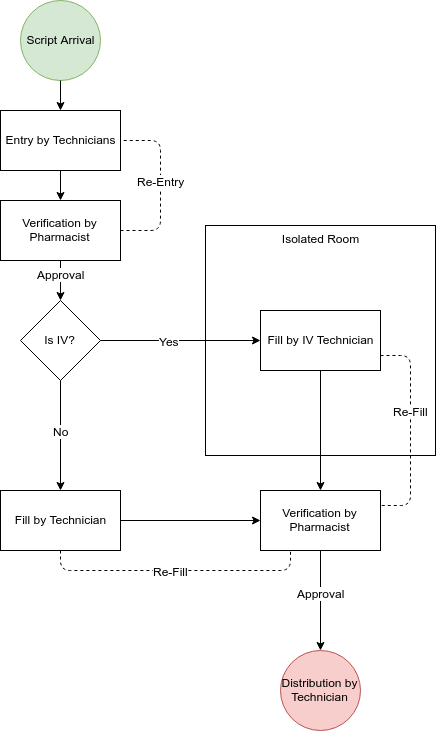
\includegraphics[scale=.5]{Flowchart.png}
\caption{Pharmacy workflow by task position noting which tasks are pharmacist only.}
\label{fig:flowchart}
\end{figure}
For our control case, we operate under the assumption that no tasks in this process have any issues with failure or delays. This is obviously a simplified case, but we shall construct the simulation in such a way that including it would be quite simple to do.  With this workflow defined, we consider the next step of building our simulation, identifying the durations of the different tasks.
\section*{Distribution Identification}
\addcontentsline{toc}{section}{Distribution Identification}
As noted above, there are six pivotal tasks that we must establish the duration of in order to effectively perform an analysis. In addition to these tasks, we are also aware of the fact that the times between incoming oral and IV orders come from different distributions. As part of the supplied data, we have samples of the completion times of each of these eight different categories, ranging in size from 34 to 60 observations. Using each of these samples, we shall construct Cullen and Frey graphs to attempt to isolate the correct distributions. These graphs will take the skewness and kurtosis of our task time samples and plot a point in the $skew^2/kurtosis$ plane which can then be mapped to potential distributions based on theoretical values for each distribution. With this set of hypothetical distributions in hand, we shall fit the data and test the goodness of fit statistic to identify the best fit.
\subsection*{Order Entry}
\addcontentsline{toc}{subsection}{Order Entry}
To begin, we consider the data provided for the order entry times. Using $R$, we construct both a histogram and a Cullen and Frey graph (Figure \ref{fig:orderEntryHistCullen}).
\begin{figure}[H]
\centering
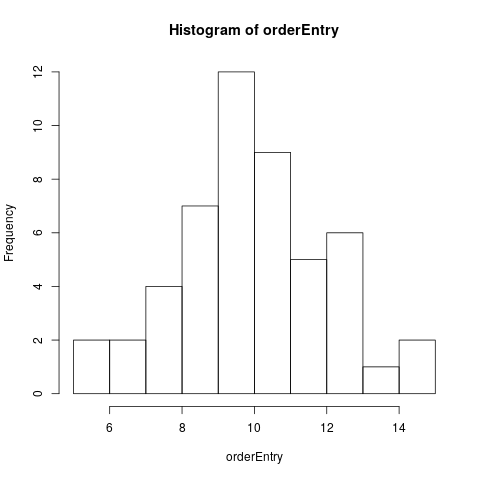
\includegraphics[scale=.35]{OrderEntryHist.png}
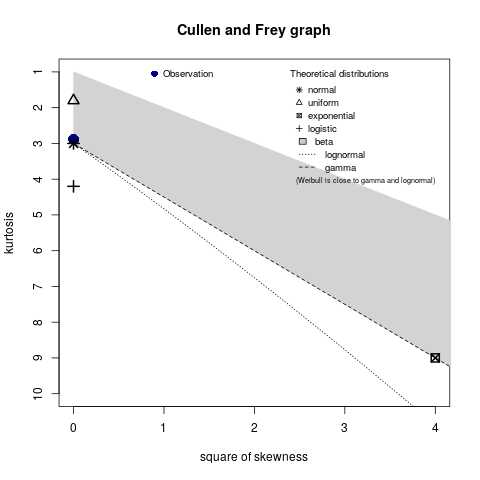
\includegraphics[scale=.35]{OrderEntryCullen.png}
\caption{Histogram of order entry times (left) and its corresponding Cullen and Frey graph (right)}
\label{fig:orderEntryHistCullen}
\end{figure}
Looking at the histogram of order entry data in Figure \ref{fig:orderEntryHistCullen}, it appears that the data comes from a normal population, and the Cullen and Frey plot supports this. For completeness, we shall test this sample as being from a normal distribution as well as a gamma and log-normal distribution, as these distributions also appear to be good potential fits in the Cullen and Frey graph. Once the data has been fit with each of these distributions, $R$ is used to compute a goodness of fit statistic, the AIC, for each model. The AIC is a sort of score for a model, which weights the accuracy of a fitted model against its own complexity. By construction, this score decreases for better models, and increases when models become too complex. This prevents over-fitting and reliance on sample data values. With this in mind, we consider the AIC scores for each of the three potential distributions for order entry below in Table \ref{table:entryGOF}
\begin{table}[H]
\centerfloat
\begin{tabular}{|r||c|c|c|}
\hline
& Normal Fit & Gamma Fit & log-normal Fit \\\hline
%Kolomogorov-Smirnov & \cellcolor{green!25}0.05172573 & 0.07123761 & 0.08600921\\\hline
%Anderson Darling & \cellcolor{green!25}0.14921512 & 0.28840960 & 0.45314418\\\hline
AIC & \cellcolor{green!25}219.8769 & 221.3501 & 223.2712\\\hline
\end{tabular}
\caption{Goodness-of-Fit statistics for hypothetical fits on the order entry data.}
\label{table:entryGOF}
\end{table}
As highlighted in Table \ref{table:entryGOF}, by treating this sample as part of a larger normal population, we produce the smallest AIC score, implying the best fit. As such, we shall treat this as the correct distribution for sampling purposes in our simulation. The relevant distribution statistics follow,
\[\text{Order Entry}\sim \text{Normal}(\mu=9.873784,\ \sigma=2.095579)\]
\subsection*{Remaining Distributions}
\addcontentsline{toc}{subsection}{Remaining Distributions}
In a similar fashion, the remaining distributions are identified as follows:
\begin{align*} 
\text{Entry Verification Times} &\sim \text{Uniform}(1.2726,\ 3.4059)\\
\text{Oral Preparation Times} &\sim \text{Lognormal}(\mu=2.99140489,\ \sigma=.06300657)\\
\text{IV Preparation Times} &\sim \text{Weibull}(shape=2.362195,\ scale=6.359247)\\
\text{Preparation Verification Times} &\sim \text{Weibull}(shape=2.911269,\ scale=2.143830)\\
\text{Dispense Times} &\sim \text{Normal}(\mu=2.947898,\ \sigma=0.566620)\\
\text{Oral Incoming Times} &\sim \text{Exponential}(\lambda = 0.129199 )\\
\text{IV Incoming Times} &\sim \text{Exponential}(\lambda = 0.05988024 )
\end{align*}
With these distributions in hand, we can begin the construction of the base case of the simulation.
%In order to effectively model and optimize the workflow in this pharmacy, we consider the given scenario, and how we might optimize it. As described, there are essentially no guidelines in place to speed up process workflow, which we will find dramatically affects the overall performance. As a pharmacy, we assume that maximizing both the number of prescriptions and the speed at which they are filled is paramount to the public image as well as its financial success.
\section*{Construction of the Base Case}
\addcontentsline{toc}{section}{Base Case}
To construct the simulation of the pharmacy, the programming language C++ was used due to its speed, as well as object oriented structure. This structure allowed for maximal customization of our data, enabling the collection of many different statistics, which we report below. To build the simulation, two unique class objects were written to house the details required for a given prescription, as well as each of the employees. Within these classes relevant structures for computing the idle times and other important statistics are included and updated throughout the simulation. An outline of the pseudo-code for the simulation follows:
\begin{verbatim}
Read in user input (number of hours, sampling frequency, number of employees, etc.)
For(each simulation){
    Construct workers and place in idle pool
    Fill queues with sample duration times from distribution data
    while(!endOfSim){
        Check and see if a new order enters in this time step
        Check if any active workers have finished task
        if(Finished){
            Push order to next queue, move employee to idle pool
        }else{
            Increment time step
        }
        For(each idle worker){
            if(any queue not empty){
                Assign task at random                   
            }else{
                Add to idle time
            }
        }
        Write queue lengths to file
    }
    Write end of simulation data
}
\end{verbatim}
With this simulation constructed, the base case was run using the following parameters,
\begin{itemize}
\item Number of Hours: 12
\item Number of Updates per Minute: 4 (Every 15 seconds)
\item Number of Pharmacists: 2
\item Number of Techs: 5 (4 Normal and 1 IV)
\item Number of Trials: 30
\end{itemize}
It is important to note here the job assignment of the base case. In this model, when job assignment begins for each employee, each non-empty task queue is put into a pool and randomly chosen with no priority. So, a pharmacist has an equal probability of doing a pharmacist only task or a technician level task. Changing this assignment will become a cornerstone of our optimization efforts. To further remove any bias in the model, the idle worker pool is shuffled randomly before each task assignment step in the simulation. This will help to alleviate any artificial effects on worker idle times.
\subsection*{Base Case Results}
Running a simulation using the parameters above, we use $R$ to analyze the output data, and obtain the following 95\% confidence intervals for various performance indicators.\\\hfill\\
First, we consider the numbers of orders that the pharmacy receives on an average day,
\begin{align*}
\text{Oral Incoming} &= [91.6024,\ 98.06426] && \text{(Number of Orders)}\\
\text{IV Incoming} &= [42.47068,\ 47.12932] && \text{(Number of Orders)}\\
\end{align*}
We see that we expect just shy of $100$ oral prescriptions, and just shy of $50$ IV orders per day. This indeed aligns with the expected values given the exponential distribution fit that was assigned to them for time between orders.\\\hfill\\
Next, we consider the average queue lengths for each task in the workflow,
\begin{align*}
\text{Entry Queue} &= [0.4310875,\ 0.6114125] && \text{(Number of Orders)}\\
\text{Entry Verification Queue} &= [7.997571,\ 12.58185] && \text{(Number of Orders)}\\
\text{Oral Fill Queue} &= [0.1240198,\ 0.1679247] && \text{(Number of Orders)}\\
\text{IV Fill Queue} &= [0.079518,\ 0.1349264] && \text{(Number of Orders)}\\
\text{Fill Verification Queue} &= [3.427384,\ 5.809907] && \text{(Number of Orders)}\\
\text{Dispense Queue} &= [0.1735777,\ 0.2304964] && \text{(Number of Orders)}\\
\end{align*}
These values tell us how many prescription orders were sitting idle at each stage of the fulfillment process, helping us identify potential bottleneck points.\\\hfill\\
Next, we consider arguably the most valuable statistic to a pharmacy from a business standpoint, the number of filled orders. 
\begin{align*}
\text{Oral Filled} &= [67.26063,\ 70.40604] && \text{(Number of Orders)}\\
\text{IV Filled} &= [32.72671,\ 37.33995] && \text{(Number of Orders)}\\
\end{align*}
We see here that we expect to fill about $70\%-75\%$ of all incoming orders. To see whether there is room for improvement in this number, we consider whether the amount of time for orders from start to finish, the ``throughput", as well as the amount of time the order sits idle leave room for improvement.
\begin{align*}
\text{Oral Throughput Times} &= [105.1253,\ 136.618] && \text{(Minutes)}\\
\text{IV Throughput Times} &= [91.9162,\ 127.0587] && \text{(Minutes)}\\
\text{Oral Wait Times} &= [68.11842,\ 99.61155] && \text{(Minutes)}\\
\text{IV Wait Times} &= [69.27191,\ 104.3281] && \text{(Minutes)}\\
\end{align*}
Here, we see that it takes an average of around two hours for an order to be filled, and over $70\%$ of this time is spent idle waiting to be selected from the queue. This would lead us to believe that there are better systems that could be implemented to increase the fill speed, and consequently the number of orders filled.\\\hfill\\
While knowing how long and how fast the orders are moving in the model is important, it is equally important for the pharmacy to measure the efficiency and use of its employees. Below, we see the estimations for how long each type of employee is idle during the simulations, expressed as a percent of the total time.
\begin{align*}
\text{Pharmacist Idle Time} &= [2.811366,\ 4.692106] && \text{(Percent of Total Time)}\\
\text{Technician Idle Time} &= [17.50725,\ 20.02053] && \text{(Percent of Total Time)}\\
\text{IV Technician Idle Time} &= [67.62806,\ 71.53167] && \text{(Percent of Total Time)}
\end{align*}
We see that as we might expect the IV technician is idle a majority of the time. This aligns with the restrictions of the job, as there are fewer IV orders received during the day, as well as the fact that the mean time to fill an IV order is under $6$ minutes. As such, there is rarely enough time for a new IV order to enter the fill queue before the technician is done with the previous task. This can also be seen above where the IV fill queue is noted to have incredibly small average lengths.\\\hfill\\
While these intervals do provide important analysis on the data, a graphical interpretation of this data will help us to more accurately examine potential points of congestion in the model. Figure \ref{fig:baseQ} has box and whisker plots for each of the average queue lengths in the base case.
\begin{figure}[H]
\centering
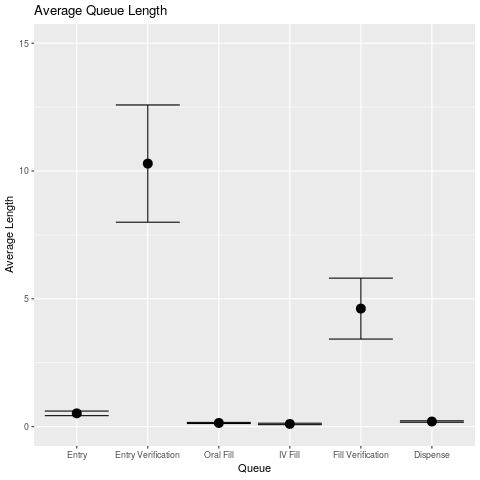
\includegraphics[scale=.5]{BaseQueueCIs.png}
\caption{Box and whisker plots for average queue lengths by type}
\label{fig:baseQ}
\end{figure}
We see that the results of this simulation point to the verification queues as being congestion points. Notably, these are the two tasks in the workflow that are pharmacist specific. This congestion then is likely due to the method by which workers received their job assignments. With the pharmacists choosing from all possible tasks equally, they can take work from the technicians, who cannot in return work from the verification tasks. This aligns with the estimated idle times from above, as we found the pharmacists to be idle significantly less than the technicians. Reducing this congestion will be the goal of our first optimization.
\section*{First Layer of Optimization}
\addcontentsline{toc}{section}{First Layer of Optimization}
With the base case of the model constructed and analyzed, we begin the first of our two pronged optimization efforts, optimizing the job choice logic to increase throughput speed, and reduce idle time in the model.
\subsection*{First Optimization: Lazy Pharmacists}
\addcontentsline{toc}{subsection}{Lazy Pharmacists}
Given that the verification tasks are causing congestion in the base model, we consider the effects of changing the job assignment method in the simulation to the following.
\begin{verbatim}
if(pharmacist){
    if(verification queues !empty){
        choose one at random
    }else{
        do nothing
    }
}
if(technician){
    if(any queues !empty){
        choose one at random
    }else{
        do nothing
}
\end{verbatim}
Under this scheme, the pharmacists will only do pharmacist specific tasks, leaving the technicians to do the remainder of the tasks. The hope is that by removing the pharmacists from the technician tasks that not only will the technician idle times be reduced, but also the lengths of the verification queues will be reduced as well. Running the simulation with the same parameters as the base case, under the new job choice logic yields some unexpected results. Firstly, the average queue lengths are much different. Figure \ref{fig:basevprof} shows the differing results.
\begin{figure}[H]
\centering
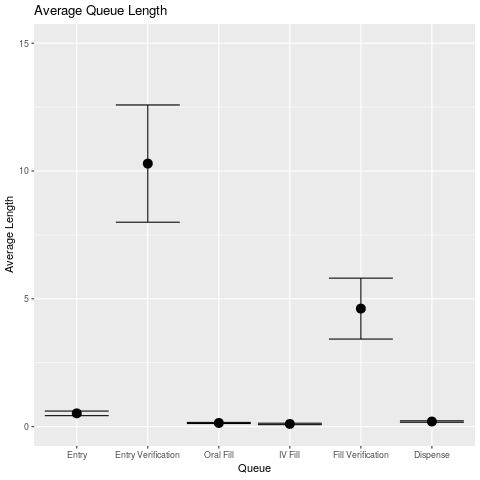
\includegraphics[scale=.35]{BaseQueueCIs.png}
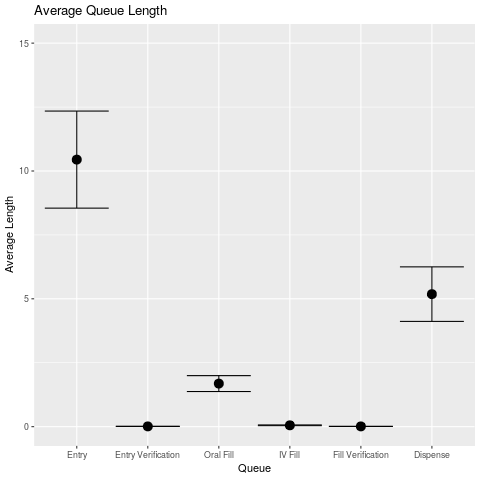
\includegraphics[scale=.35]{ProfQueueCIs.png}
\caption{Base case (left) vs. Lazy Pharmacist (Right) average queue lengths}
\label{fig:basevprof}
\end{figure}
Under the original schema, all queues were essentially empty except for the verification queues, while under our new schema all of the non-verification queues show increases, most specifically the first and last steps of the fill process. Indeed we find that the average queue length for our new case is slightly larger than before,
\[\overline{Length}_{Base}=2.648<2.898=\overline{Length}_{Lazy Pharmacist}\]
In addition to this, the average idle time for an employee is significantly larger,
\[\overline{Idle}_{Base}=14.475\% < 21.627\%=\overline{Idle}_{Lazy Pharmacist}\]
Looking more closely into this idle time data, we see that the average idle time for a pharmacist in the new scheme is approximately $67\%$, which is clearly not an effective use of their time. Before looking to see if reducing the number of pharmacists in the model would help to reduce this idle percentage, we first consider the filled order results under this scheme. Figure \ref{fig:baseprofFill} shows us a comparison in throughput.
\begin{figure}[H]
\centering
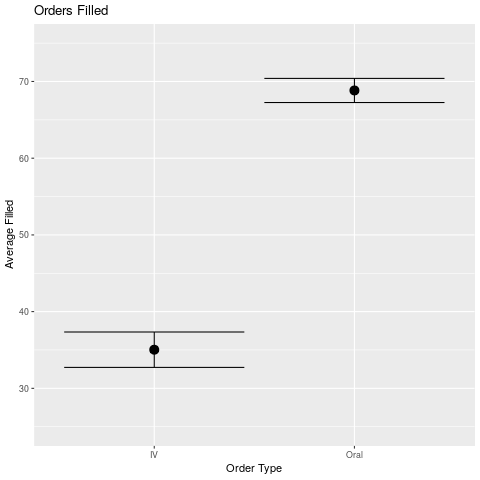
\includegraphics[scale=.35]{BaseFilledCIs.png}
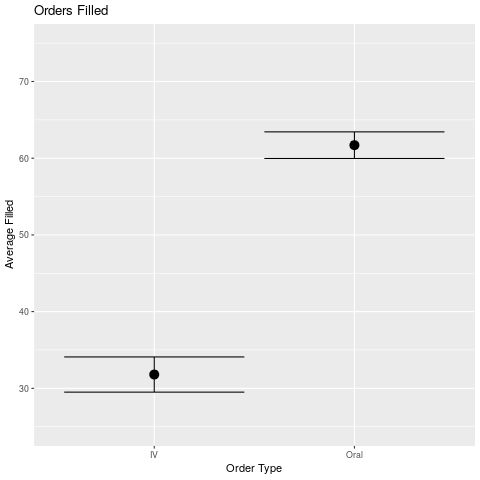
\includegraphics[scale=.35]{ProfFilledCIs.png}
\caption{Base case (left) vs. Lazy Pharmacist (Right) average number of filled orders}
\label{fig:baseprofFill}
\end{figure}
We see that in fact this method has reduced both the number of oral and IV orders that are filled over the duration of the simulation. It is likely not worth exploring further in terms of staffing optimizations as an ``over-staffed" run yielded worse results. As such, we seek to find a better process optimization.
\subsection*{Second Optimization: Largest Queue}
\addcontentsline{toc}{subsection}{Largest Queue}
Given that forcing the pharmacists to only pull from the verification tasks is hurting the efficiency of the model, we consider a new job assignment logic, choosing the most full task queue. So, a pharmacist will choose to take their next task from the largest of all five possible queues, while technicians may choose from the three technician level queues. This method should help to ensure that both employees and orders are moving as efficiently as possible as it favors maintaining the smallest possible net queue sizes. Running the simulation with the same parameters as the base case, under the new job choice logic yields results that are more aligned with what we would expect. Figure \ref{fig:basevlong} shows the comparison on average queue lengths between the base case and the longest queue method.
\begin{figure}[H]
\centering
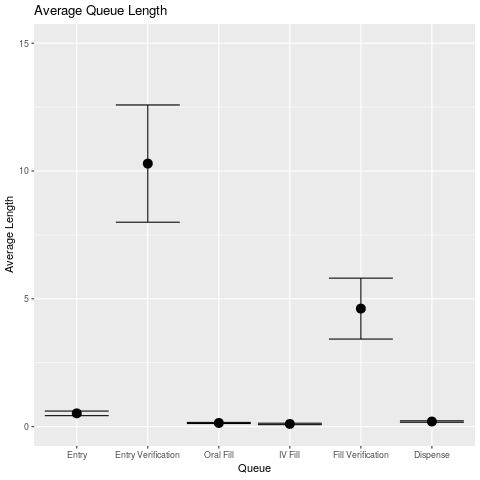
\includegraphics[scale=.35]{BaseQueueCIs.png}
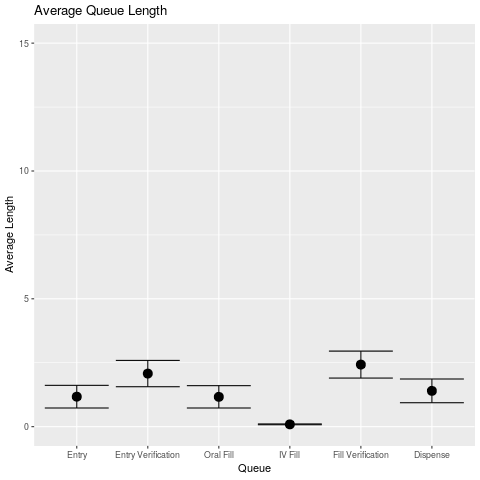
\includegraphics[scale=.35]{LongestQueueCIs.png}
\caption{Base case (left) vs. Largest Queue (Right) average queue lengths}
\label{fig:basevlong}
\end{figure}
We see that under this new system, all of the queues (except IV fill) have non-zero means, but that they are all relatively small compared to the mean of approximately 10 for the base entry verification length. Looking deeper into the data, we see that the average queue length is reduced from $2.648$ in the base case to $1.389$ in this new method. In addition to this, average idle time for the workers is reduced from $14.475\%$ in our base model to $13.395\%$. While these changes may seem somewhat small, consider now the mean throughput times between the two models.
\begin{figure}[H]
\centering
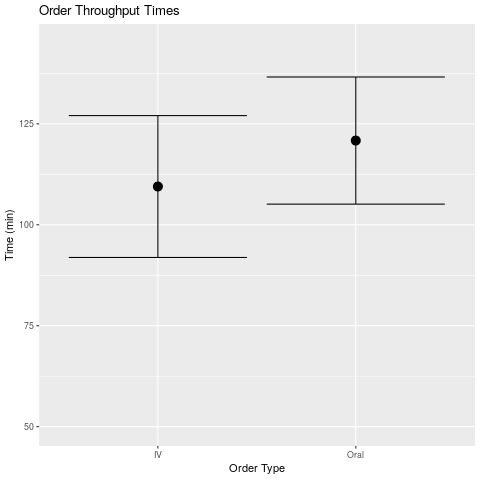
\includegraphics[scale=.35]{BaseThroughputCIs.png}
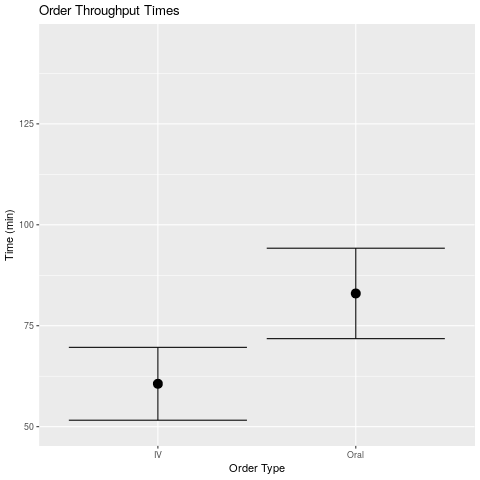
\includegraphics[scale=.35]{LongestThroughputCIs.png}
\caption{Base case (left) vs. Largest Queue (Right) average throughput times by order type}
\label{fig:basevlongthrough}
\end{figure}
We see that by choosing the longest queue as the next task, the average throughput time for an order is reduced by a factor of almost $30\%$. As we would expect, this also helps to reduce the average wait time for orders, as well as the idle times of the employees.  While this method is clearly superior to the base case, we consider finally a combination of the Lazy Pharmacist and Longest Queue methods.
\subsection*{Third Optimization: Smart Method}
\addcontentsline{toc}{subsection}{Smart Method}
As our final job assignment optimization we consider a sort of mixture between choosing the longest queue and relegating the pharmacists to the verification queues. Namely, under this schema, the pharmacist will first check to see if any of the verification queues are non-empty, and if so, they will choose the largest one. Otherwise, they choose the largest from the remaining queues. The technicians remain unchanged from before, always choosing a task from the largest queue.
\begin{verbatim}
if(pharmacist){
    if(either verification queue is nonempty){
        choose largest
    }else{
        choose largest technician level queue
    }
}
if(technician){
    choose largest technician level queue
}
\end{verbatim}
Again we implement this model with the basic parameters from before, getting again better results than before. As before, we consider the comparison between the base case and the smart method queue lengths to begin to test whether we have achieved optimization.
\begin{figure}[H]
\centering
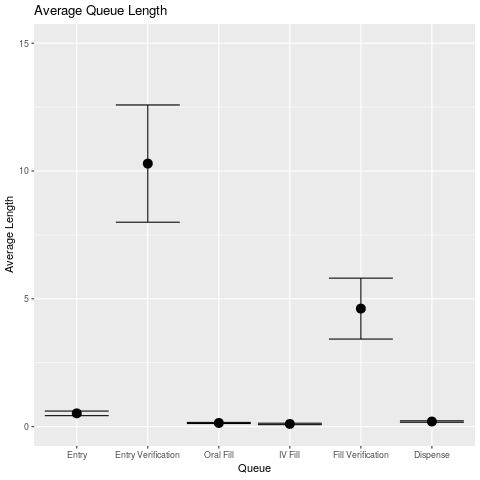
\includegraphics[scale=.35]{BaseQueueCIs.png}
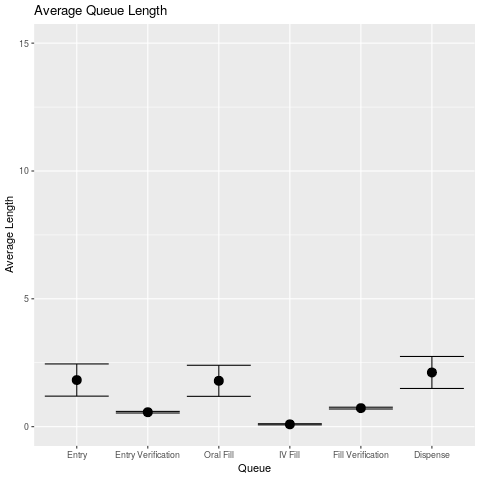
\includegraphics[scale=.35]{SmartQueueCIs.png}
\caption{Base Case (left) vs. Smart Method (Right) average queue lengths}
\label{fig:basevsmart}
\end{figure}
As with the longest queue method we see a significant reduction in the average queue length, going from $2.6475$ in the base case to $1.1869$ under the smart method. Since we have established that the longest queue is our front-runner for the optimization, we shall also use it as a basis for comparison for this smart method. Figure \ref{fig:longvsmart} contains the comparison between the average queue lengths for these two methods.
\begin{figure}[H]
\centering
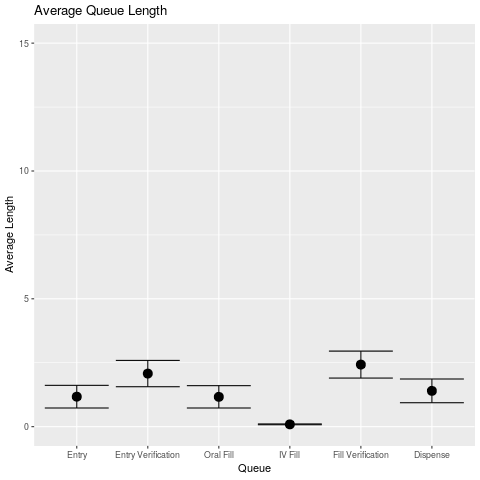
\includegraphics[scale=.35]{LongestQueueCIs.png}
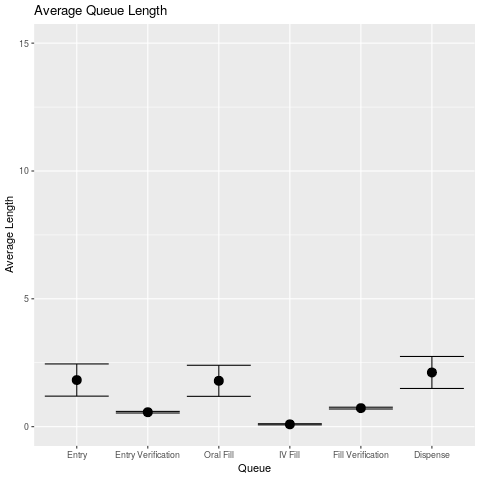
\includegraphics[scale=.35]{SmartQueueCIs.png}
\caption{Longest Queue (Left) vs. Smart Method (Right) average queue lengths}
\label{fig:longvsmart}
\end{figure}
As expected based on the results of the lazy pharmacist method, we see improvement in the size of the verification queue lengths at the slight cost to the remainder of the queue lengths. Looking into the data we find,
\[\overline{Length}_{Longest}=1.389 > 1.187 = \overline{Length}_{Smart}\]
\[\overline{Throughput}_{Longest}=71.813 > 64.920 = \overline{Throughput}_{Smart}\]
It would appear that we have achieved a slight increase in effectiveness with this new implementation, but it is hard to say given the relative magnitudes of the standard deviations in the data, thus further analysis is required.
\section*{Comparing the First Stage Optimizations}
\addcontentsline{toc}{section}{Comparing First Stage Optimizations}
Given that a pharmacy is a business above all else, the goal of these optimizations should be to increase the number of orders filled and reduce the employee idle times as much as possible. As such, we shall conduct a one-way ANOVA test on the mean number of orders filled to find the most effective model under the given conditions. Looking first at the IV filled data across the different methods, we see no marked difference among the four, they are all within one standard deviation of each other. As such, we shall focus on the oral filled data, as there is more significant variation in the results. First, let us consider a collation of the oral filled data across the methods, Table \ref{table:collate}.
\begin{table}[H]
\centerfloat
\begin{tabular}{|r||c|c|c|}
\hline
Method & Mean & Standard Deviation & $n$\\\hline\hline
Base Case & $68.8$ & $4.40$ & $30$\\\hline
Lazy Pharmacist & $61.7$ & $4.85$ & $30$\\\hline
Largest Queue & $73.3$ & $9.18$ & $30$\\\hline
Smart Method & $78.4$ & $6.04$ & $30$\\\hline
\end{tabular}
\caption{Collation of the Oral Fill data for each of the different optimization methods}
\label{table:collate}
\end{table}
While Table \ref{table:collate} allows us to see the numbers, it is more useful to see the difference in a graphical form as in Figure \ref{fig:anovaBox}.
\begin{figure}[H]
\centering
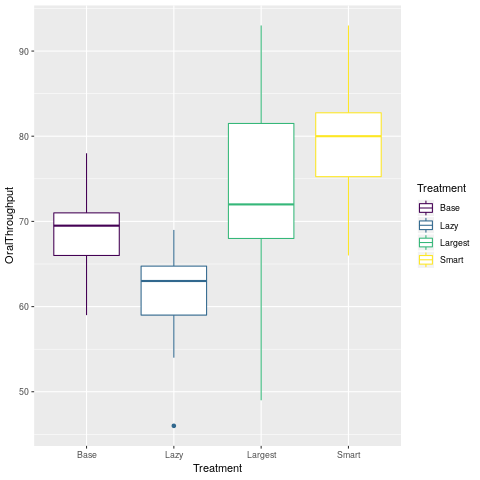
\includegraphics[scale=.5]{anovaBox.png}
\caption{Box plots for the Oral Fill data in each method}
\label{fig:anovaBox}
\end{figure}
We see from Figure \ref{fig:anovaBox} that there does seem to be a difference among the models, though it is hard to confirm visually, especially for the longest queue and smart methods. Running the ANOVA test on the null hypothesis of $\mu_i=\mu_j\ \forall i,j\in\text{Methods}$, we arrive at the $F$ statistic, 
\[F=36.96\Rightarrow p<2\times10^{-16}\]
which is highly significant. Given that this $p$ value is far less than our standard cutoff of $\alpha = 0.05$, we reject the null hypothesis in favor of the alternative, that there is a difference in at least one of the means. Given this result, we shall use $R$ to compute the Tukey honest significant differences between the means, whose results can be found in Table \ref{table:tukey}.
\begin{table}[H]
\centerfloat
\begin{tabular}{|r||c|c|}
\hline
Methods & Difference & $p$-value\\\hline\hline
Lazy-Base   &  $-7.133333$ & $0.0001922$\\\hline
\cellcolor{yellow!25}Largest-Base  & \cellcolor{yellow!25}$4.500000$ & \cellcolor{yellow!25}$0.0367813$\\\hline
Smart-Base  &   $9.600000$ & $0.0000003$\\\hline
Largest-Lazy & $11.633333$ & $0.0000000$\\\hline
Smart-Lazy  &  $16.733333$ & $0.0000000$\\\hline
\cellcolor{yellow!25}Smart-Largest & \cellcolor{yellow!25}$5.100000$ & \cellcolor{yellow!25}$0.0132541$\\\hline
\end{tabular}
\caption{Tukey HSD for different method means}
\label{table:tukey}
\end{table}
The results in Table \ref{table:tukey} are essentially pairwise $t$-tests to compare the means of each methods oral throughput. Note, Table \ref{table:tukey} has two rows highlighted. These rows correspond to the differences between the base method and largest queue method, as well as the largest queue method to the smart method. Using our standard $\alpha=0.05$, we can draw the following conclusion comparing the different methods,
\[\text{Smart $>$ Largest $>$ Base}\]
Note, this alpha comparison does not require a Bonferroni correction, as $R$ computes the adjusted $p$-value to correct for the multiple comparisons taking place. From these results, we see that while the largest queue did provide significant improvement over the base case, the smart method provided a significant improvement over the largest method. As such, we shall treat the smart method as the ``optimal" method for the next stage of our optimization efforts, improving staffing efficiency.
\section*{Efficiency Mesh}
\addcontentsline{toc}{section}{Efficiency Mesh}
Up until this point, all of our analysis has been performed on the basic assumptions from the base case,
\begin{itemize}
\item Number of Hours: 12
\item Number of Updates per Minute: 4 (Every 15 seconds)
\item Number of Pharmacists: 2
\item Number of Techs: 5 (4 Normal and 1 IV)
\item Number of Trials: 30
\end{itemize}
While this may be the current conditions of the pharmacy, it is still possible that this is not the most cost effective staffing. In order to determine the best possible configuration of employees, we shall construct a $10\times 10$ mesh that defines the pharmacies profit as a function of the number of employees of each type. Here, each point in our mesh corresponds to a coordinate in the Technician-Pharmacist plane that has a magnitude of profit. In order to assure fairness, the simulation is run with the same time distribution sampling inputs for each coordinate configuration, and run 30 times to allow for random variance in choosing queues to be accounted for. Let us define the profit function as,
\[\mathcal{P}=\mathcal{V}(Filled_{Oral}+Filled_{IV})-\mathcal{C}_{P}(n_{P})-\mathcal{C}_{T}(n_{T})\]
That is to say, the pharmacy profit for a given employee configuration is revenue per filled order times the number of filled orders less the cost of employees in the configuration. Where $\mathcal{V}$ is the revenue per filled prescription, $n_P$ and $n_T$ are the numbers of pharmacists and technicians in the model, and $\mathcal{C}_P$ and $\mathcal{C}_T$ is the cost per employee of both types.  From the salary reporting website Glassdoor, we obtain yearly salary data for both pharmacists and pharmacy technicians, and scale it to get an approximate cost for a 12 hour shift in terms of salary \cite{PSalary}\cite{TSalary}. Additionally, the average per-prescription revenue is estimated to be $\$55.99$ based on data from 2016 \cite{Revenue}. With this data in hand, we may write the profit function as,
\[\mathcal{P}=\$55.99(Filled_{Oral}+Filled_{IV})-\$748.58(n_{P})-\$161.58(n_{T})\]
Using the Smart Method developed earlier, we evaluate $\mathcal{P}$ over the mesh of staffing ``coordinates" in order to create a 3-D surface that describes the profit. This surface is then projected onto a 2-D heat-map weighted by profit in Figure \ref{fig:heatmap}.
\begin{figure}[H]
\centering
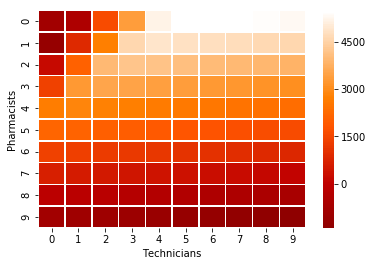
\includegraphics[scale=.75]{profitheatmap.png}
\caption{Heatmap of profit values using the Smart Method. Note, labeling on the $x$ and $y$ axes is reduced by one due to indexing.}
\label{fig:heatmap}
\end{figure}
As evidenced by the heat map, we see that the most profitable configurations occur for low numbers of pharmacists and higher numbers of technicians to compensate.  In fact, we find that the optimal number of employees for this test is one pharmacist and six technicians (5 normal and 1 IV). This resulted in an estimated net profit of $\mathcal{P}(1,6)=\$4894.02$ per day, though most of the surrounding mesh points had an approximately similar value, most specifically when moving along the technician axis.\\
This being said, there are a number of potential issues with this efficiency mesh. It makes broad assumptions about the value of each filled order, as well as approximate salary data. These approximations could be improved using real world data that the pharmacy would be able to provide, as well as the addition of specific salary data. This being said however, due to the massive discrepancy between the salary of pharmacists as opposed to technicians, it is unlikely that the ideal configuration will deviate all that much from our approximation.
\section*{Conclusions}
\addcontentsline{toc}{section}{Conclusions}
After performing both layers of optimization, we discovered a number of different effects that simple changes to task logic and staffing caused. While altering the task choice logic for the pharmacists and main technicians had dramatic effects on the overall effectiveness of the pharmacy, we noted that there was a minimal effect on the IV Technicican. In addition, we noticed that regardless of task prioritization method, as overall efficiency increased, the idle times of all employees decreased, while maintaining the trend that pharmacists had less idle time than technicians. This is likely due to the fact that they have a larger range of tasks to pull from, as well as the chance to steal a task from a technician.
%we see that there is a large range of efficiencies possible for this pharmacy. As we found before, simple workflow management methods could be implemented to reduce average throughput time by nearly a third, as well as reduce employee idle times...\\
\section*{Further Studies}
\addcontentsline{toc}{section}{Further Studies}
\subsection*{Data Improvements}
\addcontentsline{toc}{subsection}{Data Improvements}
As we discovered during our analysis, there are many points in this simulation that rely on estimates based on a small amount of data, namely our time distributions for the base case. In addition to these estimations, a number of important model effects are omitted due to the lack of data provided. Below, we suggest a number of potential improvements to this data.
\subsubsection*{Time Distribution Updates}
\addcontentsline{toc}{subsubsection}{Time Distribution Updates}
During the construction of our models, we used small sample sets of time data to estimate population distribution parameters. As such, we potentially ran the risk of under fitting the data, or estimating from fringe data sample cases. Larger samples of time data would help us to more accurately get a true estimation of the actual time population parameters.  Additionally, our model does not allow for employee skill and experience to be factored into the processes at all. It seems likely that a pharmacist would have more experience at performing technician level tasks, as they likely were employed as technicians before becoming pharmacists. This experience likely translates into faster task completion times, which our model does not account for. In this same vein, it is also likely that the incoming order rate is not a constant distribution, but rather a time sensitive process. Given that the Mayo Clinic has three main campuses in differing regions of the country, the levels of prescription needs are likely quite different. It is likely that more prescriptions are filled during the winter months in the Minnesota area due to an increase in hospitalizations due to vehicle accidents during inclement weather, as well as cold weather related sicknesses; whereas in Florida, there are probably more medications filled for long term conditions like hypertension and blood pressure management due to an older population base, and less winter effects to consider. As such, data specific to each region should be included into the model for optimal results.
\subsubsection*{Other Model Effects}
\addcontentsline{toc}{subsubsection}{Other Model Effects}
In addition to the potential issues with the time distribution estimates, there are also a number of human factors that were omitted for simplicity in this study that could potentially be addressed with more data. These factors include,
\begin{itemize}
\item Failed verification tasks requiring a task to be re-done.
\item Employee breaks and shift changes.
\item Leftover prescriptions in various queues from previous day.
\item Order cancellation/changes.
\item Impedance by customers (Complaints or questions that occupy an employee for an extended period of time)
\end{itemize}
By construction, our model could easily be adapted to include the effects of these factors, using similar techniques to parameter estimation as before. This data could be collected and continually updated over time, so that the model is kept current and effective as needs change in the future.

\begin{thebibliography}{9}
\bibitem{georgetown} ``Prescription Drugs.” \textit{Health Policy Institute}, \url{hpi.georgetown.edu/rxdrugs/}.
\bibitem{statistica} Statista Research Department. ``U.S. Average Number of Prescriptions per Capita.” \textit{Statista}, 9 Aug. 2019, \url{www.statista.com/statistics/315476/prescriptions-in-us-per-capita-by-age-group/}.
\bibitem{PSalary} ``Salary: Pharmacist.” \textit{Glassdoor}, \url{www.glassdoor.com/Salaries/pharmacist-salary-SRCH_KO0,10.htm}.
\bibitem{TSalary} ``Salary: Pharmacy Technician.” \textit{Glassdoor}, \url{www.glassdoor.com/Salaries/pharmacy-technician-salary-SRCH_KO0,19.htm}.
\bibitem{Revenue} Fein, Adam J. ``New Data: Pharmacy Owners' Profits Fall As Industry Competition Rises.” \textit{Drug Channels}, 9 Jan. 2018, \url{www.drugchannels.net/2018/01/new-data-pharmacy-owners-profits-fall.html}.
\end{thebibliography}
\end{document}                          % The required last line
